\documentclass[10pt]{beamer}

% \usepackage{beamerthemesplit} // Activate for custom appearance

\title{Credit Rationing\\\large Perspectives on Economics TA Sessions}
\author{Qing Zhang}
\institute{Columbia University}
\date{\today}

\begin{document}

\frame{\titlepage}

\frame{
\frametitle{Overview}
\begin{itemize}
\item Why is credit typically rationed (more people want to borrow at the current interest rate than can be satisfied)? Why does the interest rate not rise to clear the market?
\item Stiglitz and Weiss, Credit Rationing in Markets with Imperfect Information
\item Similar question about unemployment last time. Similar answer: interest rate could change the quality of loans. 
\begin{itemize}
\item The interest rate that maximizes banks' profit is not necessarily the interest rate that clears the market.
\item Even though the bank could raise interest rate and still make loans, those loans have higher risks that result in lower expected return. 
\item Therefore the bank is not willing to raise interest rate. 
\end{itemize}
\end{itemize}
}

\frame{
\frametitle{Idea}
\begin{figure}
\centering
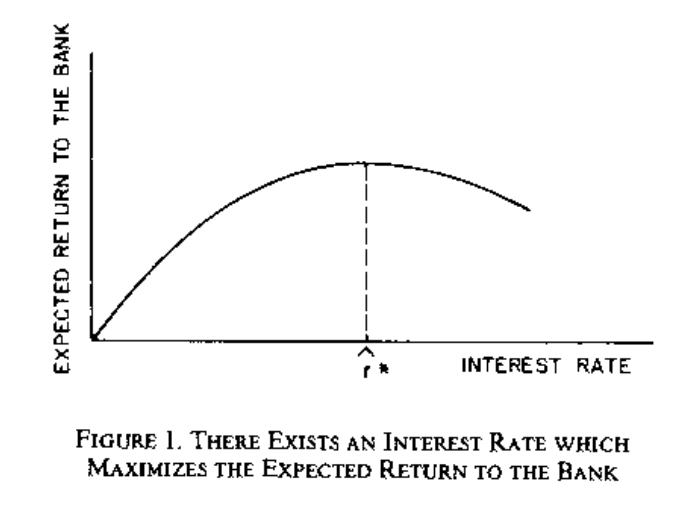
\includegraphics[width = 0.5\textwidth]{hump}
\end{figure}
They discuss two types of credit rationing in this paper:
\begin{itemize}
\item Among identical loan applicants, some receive a loan and others do not.
\item There are identifiable groups of people who are unable to obtain loans at any interest rate.
\end{itemize}
}

\frame{
\frametitle{Idea: Shapes of Payoffs}
\begin{itemize}
\item Borrower borrows amount $B$, which carries interest rate $\hat{r}$. 
\item If return of the project $R$ is higher enough, the borrower can pay back $B(1+\hat{r})$ in full. 
\item If the return turns out to be not high enough, the borrower only pays whatever the return is, plus collateral $C$.
\item Therefore borrower's profit is 
\[\pi(R, \hat{r}) = \text{max} (R-(1+\hat{r})B, -C)\]
which is bounded below by $-C$. 
\end{itemize}
}

\frame{
\frametitle{Idea: Shapes of Payoffs}
\begin{figure}
\centering
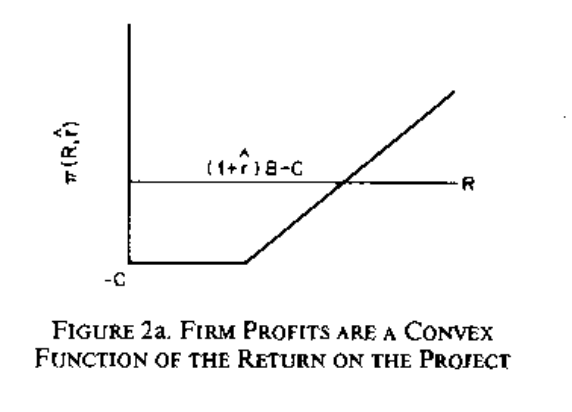
\includegraphics[width = 0.6\textwidth]{borrow_return}
\end{figure}
\begin{itemize}
\item From the graph, we see that borrower's profit is a convex function of $R$. 
\item By Jensen's inequality, for distributions of $R$ with equal mean, a more disperse distribution (higher risk) entails higher expected profit.
\end{itemize}
}

\frame{
\frametitle{Idea: Shapes of Payoffs}
\begin{itemize}
\item On the flip side, the bank gets $B(1+\hat{r})$ when borrower is able to fully repay. 
\item When borrower cannot fully repay, the bank gets $R+C$.
\item Therefore bank's return is given by
\[\rho(R, \hat{r}) = \text{min} (R+C, B(1+\hat{r}))\]
which is bounded above by $B(1+\hat{r})$.
\end{itemize}
}

\frame{
\frametitle{Idea: Shapes of Payoffs}
\begin{figure}
\centering
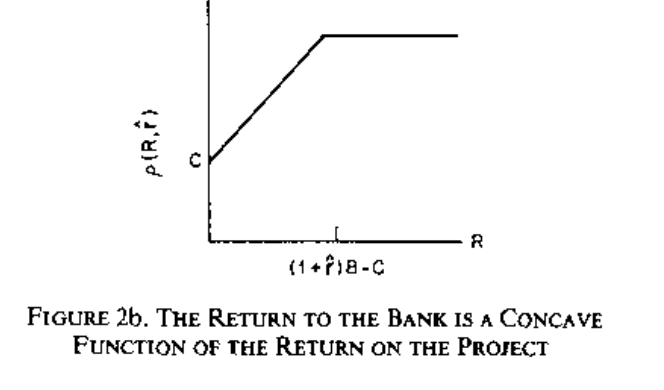
\includegraphics[width = 0.7\textwidth]{lend_return}
\end{figure}
\begin{itemize}
\item Bank's return is a concave function of $R$. 
\item By Jensen's inequality, for distributions of $R$ with equal mean, a more disperse distribution (higher risk) entails lower expected return for the bank.
\end{itemize}
}

\frame{
\frametitle{A Little Formalization}
\begin{itemize}
\item Return of a project $R$ has c.d.f. $F(R, \theta)$, where higher $\theta$ indexes higher risk. 
\item \textbf{Theorem 1}: For a given interest rate $\hat{r}$, there is a critical value $\hat{\theta}$ such that a firm borrows from the bank if and only if $\theta > \hat{\theta}$.
\item This follows immediately from Jensen's inequality. Intuition: higher-risk firms benefit more from the limited liability repayment $R+C$. 
\item The threshold $\hat{\theta}$ satisfies 
\[\Pi(\hat{r}, \hat{\theta}) = \int_0^\infty \text{max} (R-(1+\hat{r})B, -C)dF(R, \hat{\theta}) = 0\]
expected profit equals 0.
\end{itemize}
}

\frame{
\frametitle{Model}
\begin{itemize}
\item \textbf{Theorem 2}: As the interest rate increases, $\hat{\theta}$ increases. 
\item As interest rate increases, expected profit of all firms decrease. Only higher-risk firms are able to maintain a positive expected profit. 
\item Formally,
\[\frac{d\hat{\theta}}{d\hat{r}} = \frac{B\int_{(1+\hat{r})B-C}^\infty dF(R, \hat{\theta})}{\partial \Pi/\partial \hat{\theta}} > 0\]
This follows directly from applying the implicit function theorem.
\item \textbf{Theorem 4}: If there are a discrete number of potential borrowers each with a different $\theta$, bank's mean expected return will not be a monotonic function of $\hat{r}$. 
\end{itemize}

}

\frame{
\frametitle{A Two-Type Example}
\begin{figure}
\centering
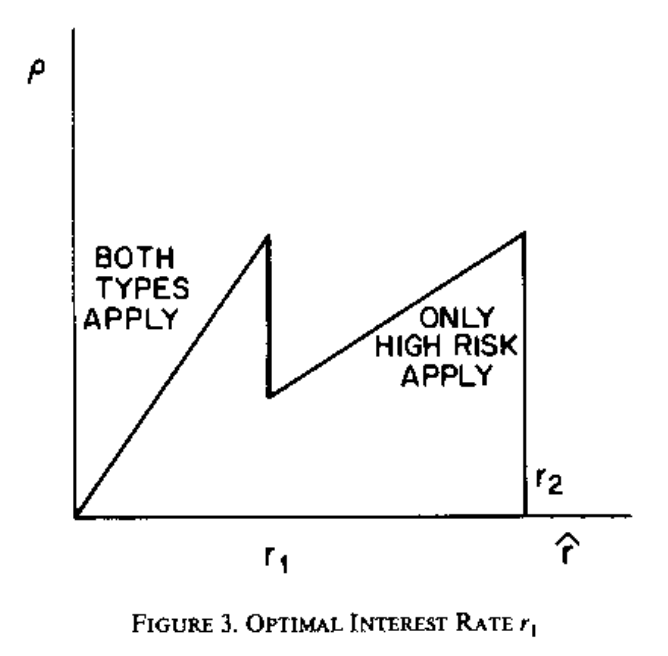
\includegraphics[width = 0.5\textwidth]{nonmonotone}
\end{figure}
When the low-risk type drops out, there is a discrete fall in bank's mean return. 

}

\frame{
\frametitle{Credit Rationing}
\begin{itemize}
\item \textbf{Theorem 5}: Whenever $\bar{\rho}(\hat{r})$ has an interior mode, there exists supply functions of funds such that competitive equilibrium entails credit rationing. 
\item We assume the supply of funds is determined by depositors' response to the return of loans. 
\item Not saying there must be credit rationing, but there can be credit rationing. 
\end{itemize}

}

\frame{
\frametitle{Credit Rationing}
\begin{figure}
\centering
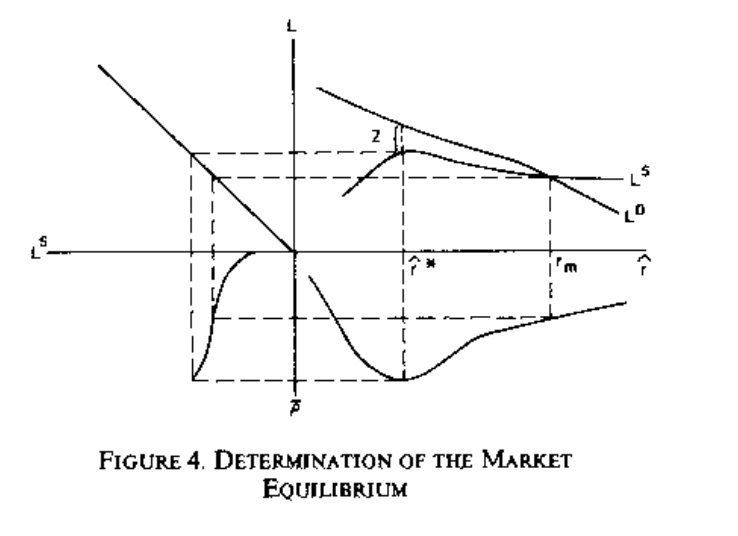
\includegraphics[width = 0.6\textwidth]{eqm}
\end{figure}
\begin{itemize}
\item $\hat{r}^*$ is equilibrium interest rate, $z$ is equilibrium excess demand of loans. 
\item Now suppose the supply of funds increase, this could absorb the excess demand without moving interest rate at all.
\item When supply of funds increases further, interest rate will go down (we have assumed that the banking sector is competitive throughout).
\end{itemize}

}

\frame{
\frametitle{Distinguishable Borrowers}
\begin{itemize}
\item Now suppose banks have a little bit more information: they can distinguish between a number of groups of people, but not borrower risks within the same group. 
\item Each group has an interest rate at which the mean expected return is maximized. 
\item Order the groups so that for $i>j$, $\text{max} \rho_i(\hat{r}_i) > \text{max} \rho_j(\hat{r}_j)$, i.e., the higher groups are more profitable for the bank. 
\end{itemize}
}

\frame{
\frametitle{Distinguishable Borrowers}
\begin{itemize}
\item \textbf{Theorem 14}: The equilibrium interest rates are such that for all $i, j$ receiving loans, $\rho_i(\hat{r}_i) = \rho_j(\hat{r}_j)$.
\item Suppose banks are making more profit off of group $i$ than group $j$. Then banks will compete to lend to group $i$, lowering interest rate (and hence profit) charged to group $i$.
%\item \textbf{Theorem 13}: For $i>j$, type $j$ borrowers will only receive loans if credit is not rationed for type $i$ borrowers.
%\item In other words, there is a strict order in which the groups' demand for credit is satisfied. 
\end{itemize}
}

\frame{
\frametitle{Graphical Representation}
\begin{figure}
\centering
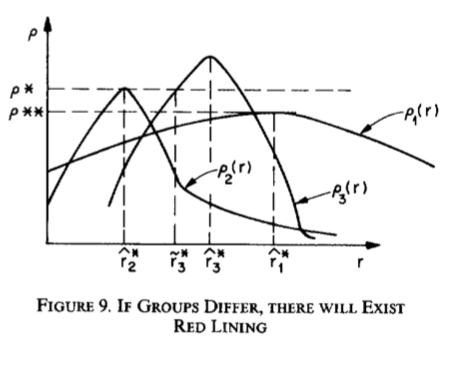
\includegraphics[width = 0.6\textwidth]{redline}
\end{figure}
\begin{itemize}
\item Starting from the highest peak in $\rho_3(r)$, we gradually walk down the hill as the supply of funds increases. 
\item Say when the market-wide return is $\rho^*$ the supply of funds is depleted. This means interest rate charged to group 2 is $\hat{r}^*_2$, and interest rate charged to group 3 is $\tilde{r}^*_3$.
\end{itemize}
}

\frame{
\frametitle{Graphical Representation}
\begin{itemize}
\item Group 3 borrowers who are willing to borrow at interest rate above $\tilde{r}^*_3$ are not rationed. Group 2 borrowers who are willing to borrow at $\hat{r}^*_2$ may be rationed. 
\item In this situation group 1 borrowers cannot borrow at any interest rate. They are simply not as profitable as groups 2 and 3 from the point of view of banks.
\item However, investing in group 1 may be more profitable than groups 2 and 3 from a social point of view. Recall that (when the project is successful) banks do not capture the returns $R$, but only a fixed repayment. 
\item Consequently, there is a mismatch between social returns and returns to banks. 
\end{itemize}
}


\end{document}